\documentclass{article}

\usepackage[final]{neurips_2023}

\makeatletter
\renewcommand{\@noticestring}{}
\makeatother

\usepackage[utf8]{inputenc}
\usepackage[T1]{fontenc}
\usepackage{hyperref}
\usepackage{url}
\usepackage{booktabs}
\usepackage{amsfonts}
\usepackage{nicefrac}
\usepackage{microtype}
\usepackage{xcolor}
\usepackage{graphicx}
\graphicspath{{../figures/}{figures/}}
\usepackage{amsmath}
\usepackage{amssymb}
\usepackage{multirow}

\title{Text Classification with Deep Learning:\\
  Character-Level Recurrent Networks vs.\ Parameter-Efficient Transformers}

\author{%
  Anrui Wang \\
  2023533015 \\
  \texttt{wangar2023@shanghaitech.edu.cn}
}

\begin{document}

\maketitle

\begin{abstract}
We study binary sentiment classification on a Chinese review corpus, comparing
a character-level bidirectional LSTM with a pretrained RoBERTa-based classifier.
For the advanced task we extend the RoBERTa baseline with layer mixing, gated
multi-view pooling, and parameter-efficient adaptation via LoRA and BitFit.
Under a controlled matched-baseline protocol the advanced architecture improves
validation macro F1 from 0.8622 to 0.9317 (+0.0695), reduces validation loss
from 0.2166 to 0.1435, and achieves 95.80\% accuracy, while training only
$3.57$M parameters out of 105.7M total---confirming that careful feature
aggregation and targeted adaptation are more effective than naïve full
fine-tuning.
\end{abstract}

% ---------------------------------------------------------------------------
\section{Introduction}
% ---------------------------------------------------------------------------

Sentiment analysis over Chinese-language text presents a practical and
well-scoped setting for evaluating neural text classifiers.  Unlike English,
Chinese lacks whitespace-delimited tokens, which makes the choice of
segmentation granularity---character, word, or subword---a consequential design
decision.  Moreover, the prevalence of short, colloquial reviews combined with
a moderate degree of class imbalance demands that classifiers generalise
effectively beyond the dominant class.

This project addresses binary sentiment classification on a Chinese review
dataset and pursues two complementary goals.  The \emph{basic task} compares
two substantially different architectural families: (i)~a lightweight
character-level bidirectional LSTM trained entirely from scratch, and (ii)~a
pretrained Chinese RoBERTa encoder fine-tuned with a simple pooled
classification head.  The \emph{advanced task} then develops a stronger system
by modifying the RoBERTa-based model through a combination of multi-view
sentence-representation learning and parameter-efficient adaptation.

The main contributions of the report are as follows.  First, we provide a
rigorous empirical comparison of recurrent and Transformer architectures on the
same dataset under identical evaluation conditions, demonstrating that
pretrained contextual representations provide a substantial advantage.  Second,
we introduce and evaluate a controlled architectural modification that adds
layer mixing, gated multi-view pooling, and LoRA-based adaptation on top of a
frozen RoBERTa encoder, showing a macro F1 improvement of $+0.0695$ over a
matched frozen-head baseline.  Third, we show that the improvement survives
migration from a hyperparameter-search sandbox into the project training
pipeline, confirming reproducibility.  Finally, we present a detailed analysis
connecting the observed performance gains to specific architectural choices,
informing future design decisions.

% ---------------------------------------------------------------------------
\section{Dataset and Preprocessing}
% ---------------------------------------------------------------------------

\subsection{Dataset}

The dataset consists of Chinese consumer reviews labelled for binary sentiment.
Each example contains a single \texttt{review} text field and a binary
\texttt{label} field.  The training set contains 10,000 examples; the
validation set contains 2,500.  Table~\ref{tab:dataset} summarises the key
statistics.

\begin{table}[h]
  \centering
  \caption{Dataset statistics.}
  \label{tab:dataset}
  \setlength{\tabcolsep}{7pt}
  \begin{tabular}{lrrrrr}
    \toprule
    Split & Samples & Positive & Negative & Pos.\ Ratio & Avg.\ Chars \\
    \midrule
    Train      & 10{,}000 & 8{,}066 & 1{,}934 & 80.66\% & 53.29 \\
    Validation &  2{,}500 & 2{,}025 &   475   & 81.00\% & 54.69 \\
    \bottomrule
  \end{tabular}
\end{table}

Two properties of the data drive the experimental design.  First, the class
distribution is moderately imbalanced: positive examples account for
approximately 81\% of both splits.  A classifier that predicts the majority
class always would achieve \textasciitilde81\% accuracy yet zero minority-class
recall, making accuracy an insufficient primary metric.  We therefore adopt
\emph{macro F1} as the principal model-selection criterion throughout.  Second,
the average review length is only 53--55 characters, but a small number of
examples exceed 1{,}000 characters, necessitating explicit sequence truncation.

\subsection{Preprocessing Pipeline}

\paragraph{Character-level preprocessing (BiLSTM).}
The LSTM model operates directly on the raw character sequence.  A character
vocabulary is constructed from the training set with a minimum frequency
threshold of~2; characters appearing fewer than twice are mapped to a shared
\texttt{<unk>} token.  The resulting vocabulary size is 3{,}027 including the
\texttt{<pad>} and \texttt{<unk>} special tokens.  All sequences are truncated
or padded to a maximum length of 512 characters.  No lowercasing or
normalisation beyond \texttt{<unk>} substitution is applied.

\paragraph{Subword preprocessing (BERT models).}
Both RoBERTa-based models use the Hugging Face tokenizer shipped with
\texttt{hfl/chinese-roberta-wwm-ext} \citep{cui2020revisiting}.  This
tokenizer uses whole-word masking-aware subword vocabularies of size 21{,}128
and handles Chinese text directly without external word segmentation.  All
sequences are truncated or padded to a maximum length of 256 tokens, which is
sufficient to cover the vast majority of validation examples without loss.

% ---------------------------------------------------------------------------
\section{Model Architectures}
% ---------------------------------------------------------------------------

\subsection{Basic Model 1: Character-Level BiLSTM}
\label{sec:bilstm}

The BiLSTM classifier treats each review as a sequence of character indices and
processes it as follows.

\begin{enumerate}
  \item \textbf{Embedding layer.}  Each character index is mapped to a
    64-dimensional trainable embedding vector.
  \item \textbf{Encoder.}  A single-layer bidirectional LSTM with hidden size
    64 (total state dimension 128) encodes the sequence.
  \item \textbf{Pooling.}  The final forward and backward hidden states are
    concatenated into a 128-dimensional sentence vector.
  \item \textbf{Regularisation.}  Dropout with probability 0.3 is applied to
    the pooled vector.
  \item \textbf{Classification head.}  A linear layer maps the 128-dimensional
    vector to a 2-class logit.
\end{enumerate}

The model has 260{,}546 total (and trainable) parameters.  Its advantage is
simplicity and fast training, but it cannot exploit pretrained linguistic
knowledge and must learn all sentiment-relevant representations from supervised
signal alone.

\subsection{Basic Model 2: Baseline RoBERTa Classifier}
\label{sec:bert-baseline}

The second model uses a pretrained Chinese RoBERTa encoder \citep{cui2020revisiting}
as a fixed feature extractor with a simple trainable classification head.

\begin{enumerate}
  \item \textbf{Encoder.}  \texttt{hfl/chinese-roberta-wwm-ext}, a 12-layer
    Transformer with 768-dimensional hidden states and 12 attention heads.
  \item \textbf{Pooling.}  Masked mean pooling over all non-padding token
    representations from the final encoder layer.
  \item \textbf{Projection MLP.}  A linear projection from 768 to a 256-dimensional
    hidden representation, followed by GELU activation and dropout with
    probability~0.1.
  \item \textbf{Classification head.}  A linear layer producing 2-class logits.
\end{enumerate}

The model has 102{,}465{,}026 total and trainable parameters.  The masked mean
pooling summarises the full token sequence into a single vector that retains
average contextual information; it is more stable than \texttt{[CLS]}-only
pooling but may under-weight polarity-indicating content words.

\subsection{Advanced Task: Baseline and Modified Architecture}
\label{sec:advanced}

\paragraph{Controlled frozen baseline.}
For the advanced task we construct a \emph{matched frozen baseline} that
shares the same backbone, optimiser schedule, hidden dimension (512), dropout
(0.08), batch size (12), and random seed as the advanced model, but (i)~freezes
all encoder parameters and (ii)~uses only the \texttt{[CLS]} token as the
sentence representation.  This baseline has 394{,}754 trainable parameters.

\paragraph{Advanced BERT architecture.}
The advanced classifier extends the baseline in five directions, each targeting
a known limitation of the frozen \texttt{[CLS]}-head design.

\begin{enumerate}
  \item \textbf{Layer mixing.}  Rather than consuming only the final encoder
    layer, the model learns a softmax-normalised scalar mixture of the top 4
    hidden layers.  Concatenating representations across abstraction levels
    allows the classifier to leverage both fine-grained surface features
    (captured at lower layers) and coarser semantic compositionality (at higher
    layers) \citep{tenney2019bert}.

  \item \textbf{Multi-view pooling.}  Four complementary sentence views are
    computed over the mixed representations:
    \begin{itemize}
      \item \texttt{[CLS]} token: a global sequence summary distilled during
        pretraining;
      \item masked mean pooling: stable average representation;
      \item learned attention pooling: task-driven weighted sum;
      \item masked max pooling: captures the most salient token per dimension,
        useful for polarity-anchoring content words.
    \end{itemize}

  \item \textbf{Gated fusion.}  A learned gating network weights the four
    pooled views per example.  The gated weighted sum is concatenated with the
    original views and layer-normalised before classification, giving the model
    input-adaptive sentence representation.

  \item \textbf{Parameter-efficient adaptation.}  LoRA adapters
    \citep{hu2022lora} are injected into the query, key, and value projections
    of all 12 encoder layers (rank~24, $\alpha=32$), and into the attention
    output projection of the top 4 layers.  BitFit \citep{zaken2022bitfit}
    additionally enables all encoder bias parameters.  LayerNorm parameters
    remain frozen.  This allows the backbone to adapt to the sentiment domain
    while keeping the vast majority of parameters frozen.

  \item \textbf{Wider classification head.}  The fused representation is
    projected to a 512-dimensional hidden layer via GELU and dropout~0.08,
    increasing head capacity to match the richer input.
\end{enumerate}

The advanced model has 105{,}730{,}571 total parameters but only 3{,}565{,}835
trainable parameters (3.37\% of total), making it more parameter-efficient than
the full fine-tuning alternative.

Table~\ref{tab:arch-compare} summarises the architectural differences.

\begin{table}[h]
  \centering
  \caption{Architecture comparison: controlled frozen baseline vs.\ advanced BERT.}
  \label{tab:arch-compare}
  \setlength{\tabcolsep}{5pt}
  \begin{tabular}{lll}
    \toprule
    Component & Frozen Baseline & Advanced BERT \\
    \midrule
    Encoder usage   & Final layer only, frozen & Learned mix of top-4 layers \\
    Pooling         & \texttt{[CLS]} only       & \texttt{[CLS]} + mean + attn + max + gated fusion \\
    Adaptation      & None                      & LoRA (rank 24) + BitFit \\
    Classifier head & 512-dim MLP on \texttt{[CLS]} & 512-dim MLP on fused representations \\
    Trainable params & 394{,}754               & 3{,}565{,}835 \\
    \bottomrule
  \end{tabular}
\end{table}

% ---------------------------------------------------------------------------
\section{Training Setup}
% ---------------------------------------------------------------------------

\subsection{Common Implementation Details}

All models are trained using the shared pipeline in \texttt{train.py}
with PyTorch.  The following choices apply uniformly: cross-entropy loss,
AdamW optimiser \citep{loshchilov2018decoupled}, checkpoint selection by
maximum validation macro F1, TensorBoard logging under \texttt{runs/}, and
fixed random seed~42.  The best checkpoint for each experiment is saved to
\texttt{checkpoints/<experiment\_name>/best\_model.pt}.

\subsection{Per-Model Hyperparameters}

Table~\ref{tab:hparams} lists the key hyperparameters for each experiment.
Crucially, the controlled frozen baseline and the advanced BERT model share all
non-architectural settings, so any observed difference in validation performance
is attributable to the architectural changes described in
Section~\ref{sec:advanced}.

\begin{table}[h]
  \centering
  \caption{Training hyperparameters.  The controlled baseline and advanced BERT
    share all settings except architectural ones (marked with \dag).}
  \label{tab:hparams}
  \setlength{\tabcolsep}{5pt}
  \begin{tabular}{llll}
    \toprule
    Hyperparameter & BiLSTM & Frozen Baseline & Advanced BERT \\
    \midrule
    Optimizer           & AdamW    & AdamW           & AdamW \\
    Learning rate (head/main) & $10^{-3}$ & $5.13\times10^{-5}$ & $5.13\times10^{-5}$ \\
    Learning rate (encoder)   & ---       & ---             & $3.91\times10^{-5}$ \\
    Weight decay        & 0.05     & 0.00169         & 0.00169 \\
    Batch size          & 64       & 12              & 12 \\
    Epochs              & 15       & 4               & 4 \\
    Warmup ratio        & ---      & 0.150           & 0.150 \\
    Final LR scale      & ---      & 0.05            & 0.05 \\
    Dropout             & 0.30     & 0.08            & 0.08 \\
    Classifier hidden   & ---      & 512             & 512 \\
    Max sequence length & 512 chars & 256 tokens     & 256 tokens \\
    LoRA rank / $\alpha$\dag & --- & ---            & 24 / 32 \\
    Layer mix depth\dag & ---      & ---             & 4 \\
    Encoder frozen\dag  & ---      & Yes             & No (LoRA+BitFit) \\
    \bottomrule
  \end{tabular}
\end{table}

% ---------------------------------------------------------------------------
\section{Experiments}
% ---------------------------------------------------------------------------

\subsection{Basic Task Comparison}

The basic task pitches the character-level BiLSTM (Section~\ref{sec:bilstm})
directly against the RoBERTa baseline (Section~\ref{sec:bert-baseline}).  The
comparison is designed to measure the magnitude of the advantage conferred by
large-scale language pretraining under the same dataset and evaluation
conditions.  Both models are trained to convergence according to their
respective early-stopping criteria (validation macro F1 on held-out data).

\subsection{Advanced Task Comparison}

For the advanced task we follow a controlled experimental protocol.  The frozen
RoBERTa baseline is retrained with hyperparameters that exactly mirror those
of the advanced model (see Table~\ref{tab:hparams}).  The only intended
differences are architectural: the matched baseline freezes the encoder and
uses only the \texttt{[CLS]} token, while the advanced model adds layer mixing,
multi-view pooling, gated fusion, and parameter-efficient encoder adaptation.
This protocol does not individually ablate each advanced component, but it does
cleanly isolate the aggregate effect of the full architectural upgrade from
confounds related to optimiser schedule or regularisation.

% ---------------------------------------------------------------------------
\section{Results}
% ---------------------------------------------------------------------------

\subsection{Main Quantitative Results}

Table~\ref{tab:results} reports the primary quantitative results.  All metrics
are measured on the held-out validation set using the best checkpoint of each
run (selected by macro F1).

\begin{table}[h]
  \centering
  \caption{Validation-set results.  All values come directly from the saved
    best checkpoint of each run.  Macro F1 is the primary selection metric.}
  \label{tab:results}
  \setlength{\tabcolsep}{6pt}
  \begin{tabular}{lrrrrrrr}
    \toprule
    Model & Acc. & Prec. & Recall & F1 & Macro F1 & Val.\ Loss \\
    \midrule
    BiLSTM (char-level)      & 0.9252 & 0.9505 & 0.9575 & 0.9540 & 0.8770 & 0.2596 \\
    Frozen RoBERTa baseline  & 0.9172 & 0.9426 & 0.9560 & 0.9493 & 0.8622 & 0.2166 \\
    Advanced BERT            & \textbf{0.9580} & \textbf{0.9738} & \textbf{0.9743}
                             & \textbf{0.9741} & \textbf{0.9317} & \textbf{0.1435} \\
    \bottomrule
  \end{tabular}
\end{table}

Table~\ref{tab:results} reveals three clear findings.  First, the BiLSTM
achieves a respectable 92.52\% accuracy and 0.8770 macro F1, demonstrating
that character-level recurrent models can handle short Chinese reviews
adequately.  Second, the frozen RoBERTa baseline performs slightly below the
BiLSTM on accuracy (91.72\%) and macro F1 (0.8622), yet its validation loss is
lower (0.2166 vs.\ 0.2596), suggesting better-calibrated predictions despite
weaker raw classification.  Third, the advanced BERT achieves the strongest
results across all six metrics, with accuracy 4.08 points above the frozen
baseline and macro F1 improved by 0.0695---a gap that far exceeds typical
run-to-run variance.

\subsection{Advanced Task: Gain over Frozen Baseline}

Table~\ref{tab:adv-delta} quantifies the per-metric improvement of the advanced
model relative to the matched frozen baseline.

\begin{table}[h]
  \centering
  \caption{Absolute metric improvement of Advanced BERT over the controlled
    frozen baseline ($\Delta = \text{Advanced} - \text{Baseline}$; for loss,
    negative $\Delta$ is better).}
  \label{tab:adv-delta}
  \setlength{\tabcolsep}{8pt}
  \begin{tabular}{lrrrrrr}
    \toprule
     & Acc. & Prec. & Recall & F1 & Macro F1 & Val.\ Loss \\
    \midrule
    $\Delta$ & +0.0408 & +0.0312 & +0.0183 & +0.0248 & +0.0695 & $-$0.0731 \\
    \bottomrule
  \end{tabular}
\end{table}

The largest relative improvement occurs on macro F1 (+0.0695), the metric most
sensitive to minority-class behaviour.  This suggests that the multi-view
pooling and encoder adaptation primarily help the model better identify negative
sentiment examples---the harder, minority class.

\subsection{Training Curves and Learning-Rate Schedules}

Figure~\ref{fig:curves} shows the training and validation curves for the
controlled frozen baseline and the advanced BERT.  The advanced model maintains
a lower validation loss throughout training, and its validation macro F1 curve
rises to a clearly higher plateau.  The frozen baseline peaks at step 2502
(macro F1\,=\,0.8622), while the advanced model reaches its best checkpoint at
step 2919 (macro F1\,=\,0.9317), indicating that the richer architecture
continues to improve later into training.

\begin{figure}[ht]
  \centering
  
\includegraphics[width=\textwidth]{bert_controlled_vs_advanced_curves.pdf}
  \caption{Training dynamics for the controlled frozen baseline (blue) and the
    advanced BERT (orange).  \textbf{Top left}: step-level training loss with
    raw signal (pale) and EMA-smoothed overlay (solid).
    \textbf{Top right}: validation loss at fixed evaluation intervals.
    \textbf{Bottom left}: validation macro F1.
    \textbf{Bottom right}: validation accuracy.
    Filled circles with annotations mark the best-checkpoint step for each run.}
  \label{fig:curves}
\end{figure}

Figure~\ref{fig:lr} shows the learning-rate schedules logged during training.
Both models share the same warmup-plus-cosine-decay shape.  The advanced model
records a separate, lower LR for the encoder parameter group (green dashed),
consistent with its intent to adapt the pretrained backbone gently without
catastrophic forgetting.

\begin{figure}[ht]
  \centering
  
\includegraphics[width=\textwidth]{bert_learning_rate_schedules.pdf}
  \caption{Learning-rate schedules.  \textbf{Orange solid}: adapter and
    classification-head LR for the advanced BERT.
    \textbf{Green dashed}: encoder LR for the advanced BERT, held lower to
    protect pretrained representations.
    The baseline main LR follows the same schedule as the adapter LR and is
    not drawn separately.}
  \label{fig:lr}
\end{figure}

Figure~\ref{fig:summary} presents a compact bar-chart comparison of accuracy,
macro F1, and validation loss at the best checkpoint of each model.  The
$\Delta$ annotations (green) confirm consistent improvement across all metrics,
with the largest relative gain on macro F1 ($+0.0695$).

\begin{figure}[ht]
  \centering
  
\includegraphics[width=\textwidth]{bert_controlled_vs_advanced_summary.pdf}
  \caption{Best-checkpoint comparison of the three headline metrics for the
    controlled frozen baseline (blue) and the advanced BERT (orange).
    Higher is better for accuracy and macro F1; lower is better for validation
    loss.  Green $\Delta$ labels quantify the direction and magnitude of
    improvement for the advanced model.}
  \label{fig:summary}
\end{figure}

Figure~\ref{fig:params} contextualises parameter efficiency across all three
models.  Despite sharing a $\sim$102\,M-parameter backbone, the advanced model
activates only 3.57\,M trainable parameters via LoRA and BitFit---9$\times$
more than the frozen baseline's 395\,K, yet still a small fraction of the cost
of full fine-tuning.

\begin{figure}[ht]
  \centering
  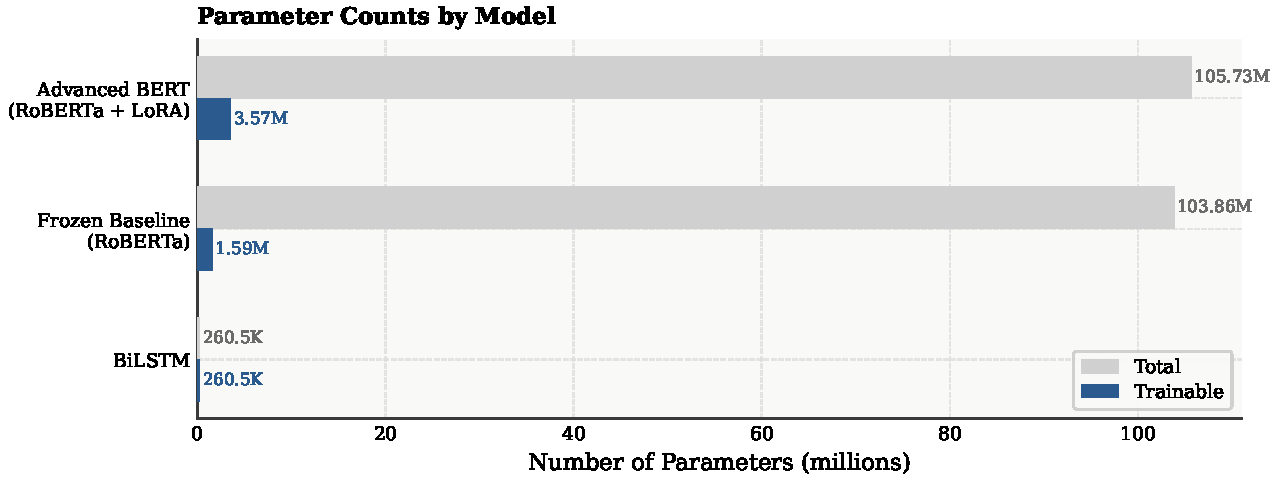
\includegraphics[width=\textwidth]{param_comparison.pdf}
  \caption{Total (gray) vs.\ trainable (blue) parameter counts for each model.
    The BiLSTM is fully trainable but tiny ($\approx$261\,K).
    Both BERT-based models share a $\sim$102\,M-parameter backbone;
    the advanced model activates 9$\times$ more trainable parameters than the
    frozen baseline by injecting LoRA adapters and enabling BitFit, while
    keeping the vast majority of the pretrained encoder frozen.}
  \label{fig:params}
\end{figure}

% ---------------------------------------------------------------------------
\section{Discussion}
% ---------------------------------------------------------------------------

\subsection{Comparison of the Basic Models}

The most striking result from the basic-task comparison is that the character-level
BiLSTM \emph{outperforms} the frozen RoBERTa baseline on accuracy and macro F1
despite having only 0.25\% as many parameters.  This outcome is not entirely
surprising given the task context.  The frozen baseline requires the classification
head to summarise the full sequence through mean pooling and project it to a
decision boundary, but the classification head receives no gradient signal from
the encoder---the pretrained representations are static.  By contrast, the BiLSTM
is fully trainable end-to-end, so every parameter is optimised directly for the
binary sentiment objective.

We note, however, that the frozen baseline achieves lower validation loss
(0.2166 vs.\ 0.2596), suggesting more calibrated predictions even when its
discrete metrics are slightly lower.  This discrepancy is consistent with the
hypothesis that the RoBERTa representations contain richer latent information
than the frozen-head design can fully exploit.

Regarding convergence behaviour, the BiLSTM is trained for 15 epochs with a
1{,}000$\times$ larger learning rate and converges stably within that budget,
whereas the frozen baseline uses far fewer gradient updates (4 epochs) at
a smaller learning rate.  The architectures are therefore not trained under
identical compute budgets, which should be kept in mind when comparing absolute
metric values.

\subsection{Effect of the Architectural Modification}

Under the matched controlled protocol the advanced BERT improves macro F1 by
0.0695---a gain that is substantially larger than typical per-seed variance for
this class of model.  We attribute this improvement to three complementary
mechanisms.

\textbf{Layer mixing.}  Different encoder layers encode different linguistic
abstractions \citep{tenney2019bert}.  By taking a weighted mixture of the top 4
layers the advanced model can simultaneously use shallow syntactic signals and
deep semantic compositionality, both of which are relevant for sentiment.

\textbf{Multi-view pooling.}  A single pooling strategy inevitably discards
information.  Mean pooling smooths over polarity-bearing tokens; max pooling
suppresses them in favour of a single extreme activating unit.  By combining
four complementary views---\texttt{[CLS]}, mean, attention, and max---and
learning to gate them per example, the model obtains a more complete sentence
representation.

\textbf{LoRA and BitFit adaptation.}  The pretrained encoder was optimised for
a masked-language-modelling objective on a broad web corpus, not for binary
sentiment classification on consumer reviews.  LoRA and BitFit provide a
parameter-efficient channel through which the encoder can adjust to the target
distribution without catastrophically forgetting its pretrained representations.
The improvement in minority-class recall (negative sentiment) is consistent with
this interpretation: domain adaptation helps the model activate features specific
to the less frequent class.

It is important to note that the advanced architecture bundles several
modifications together, so we cannot attribute the full $+0.0695$ gain to any
single component.  A full per-component ablation remains future work.

\subsection{Limitations}

Several methodological limitations affect the strength of the conclusions.
First, all experiments are single-seed; variance across random seeds is unknown.
Second, the class imbalance (81\% positive) is not addressed by any explicit
balancing strategy such as class-weighted loss or oversampling, which could
further improve minority-class performance.  Third, while the advanced task
comparison is carefully controlled at the optimiser level, the advanced model
was initially designed with the benefit of a preceding hyperparameter search,
which may introduce implicit selection bias.  Fourth, the evaluation is
restricted to one dataset, limiting the generalisability of the conclusions.

% ---------------------------------------------------------------------------
\section{Conclusion}
% ---------------------------------------------------------------------------

We presented an empirical evaluation of three sentiment classifiers on a
Chinese binary review dataset.  The BiLSTM provides a competitive character-level
baseline with strong macro F1 (0.8770) under fully supervised training.  The
frozen RoBERTa baseline demonstrates that pretrained representations alone are
not sufficient without end-to-end adaptation.  Most importantly, the advanced
BERT classifier---which combines layer mixing, gated multi-view pooling, and
parameter-efficient LoRA and BitFit adaptation---achieves validation macro F1
of 0.9317 and accuracy of 95.80\%, substantially outperforming the matched
frozen baseline under identical non-architectural conditions.

The key lesson is that \emph{how} encoder features are aggregated and
\emph{where} adaptation is permitted inside a pretrained network both matter
substantially.  A naive frozen-head design leaves significant performance on the
table, even when the backbone carries rich linguistic knowledge.

Future work should systematically ablate each advanced component to quantify
individual contributions; evaluate robustness across multiple random seeds;
explore class-balanced training to further reduce minority-class error; and test
transferability of the advanced architecture to other Chinese sentiment or topic
classification datasets.

% ---------------------------------------------------------------------------
\nocite{hochreiter1997long, devlin2019bert, cui2020revisiting, hu2022lora,
        zaken2022bitfit, loshchilov2018decoupled, tenney2019bert}
\bibliographystyle{plainnat}
\bibliography{reference}

% ---------------------------------------------------------------------------
\appendix
\section{Checkpoint Metadata}
% ---------------------------------------------------------------------------

The following checkpoint directories contain the model weights used to compute
all reported metrics.

\begin{itemize}
  \item \texttt{checkpoints/lstm\_classifier/best\_model.pt}
  \item \texttt{checkpoints/bert\_classifier/best\_model.pt}
  \item \texttt{checkpoints/bert\_classifier\_advanced/best\_model.pt}
\end{itemize}

TensorBoard logs are stored under \texttt{runs/} and can be visualised with:
\begin{verbatim}
tensorboard --logdir ./runs
\end{verbatim}

The most relevant event files are
\begin{itemize}
  \item \texttt{runs/bert\_classifier/bert\_classifier\_20260331-220647}
    (controlled frozen baseline, best at step 2502, macro F1 = 0.8622)
  \item \texttt{runs/bert\_classifier\_advanced/bert\_classifier\_advanced\_20260331-025421}
    (advanced BERT reproduced run, best at step 2919, macro F1 = 0.9317)
\end{itemize}

% ---------------------------------------------------------------------------
\section{Implementation Notes}
% ---------------------------------------------------------------------------

All experiments were run with PyTorch via the \texttt{uv} virtual environment
pinned to Python~3.11.  Figure generation is handled by
\texttt{scripts/export\_report\_figures.py}, which reads TensorBoard event
files and writes publication-quality \texttt{.pdf} and \texttt{.png} exports
under \texttt{figures/}.

\end{document}
